\documentclass{article} %\documentstyle[11pt,handout,psfig]{article}

\usepackage{fullpage,amssymb,amsmath,epsf}
\usepackage[12pt]{extsizes}

%These give really tight margins:
%\setlength{\topmargin}{-0.3in}
%\setlength{\textheight}{8.10in}
%\setlength{\textwidth}{5.8in}
%\setlength{\baselineskip}{0.1875in}
%\addtolength{\leftmargin}{-2.775in}
%\setlength{\footskip}{0.45in}
%\setlength{\oddsidemargin}{0.5in}
%\setlength{\evensidemargin}{0.5in}
%%\setlength{\headsep}{0pt}
%%\setlength{\headheight}{0pt}

%\setlength{\topmargin}{-0.5in}
\setlength{\textheight}{8in}
%\setlength{\textwidth}{5.0in}
%\setlength{\baselineskip}{0.1875in}
%\addtolength{\leftmargin}{-2.775in}
%\setlength{\footskip}{0.45in}
%\setlength{\oddsidemargin}{0.5in}
%\setlength{\evensidemargin}{0.5in}
%%\setlength{\headsep}{0pt}
%%\setlength{\headheight}{0pt}


\markright{XCS229ii}
\pagestyle{myheadings}

\newcommand{\newsec}{\section}
\newcommand{\denselist}{\itemsep 0pt\partopsep 0pt}
\newcommand{\bitem}{\begin{itemize}\denselist}
\newcommand{\eitem}{\end{itemize}}
\newcommand{\benum}{\begin{enumerate}\denselist}
\newcommand{\eenum}{\end{enumerate}}

\newcommand{\fig}[1]{\private{\begin{center}
{\Large\bf ({#1})}
\end{center}}}

\newcommand{\cpsf}[1]{{\centerline{\psfig{#1}}}}
\newcommand{\mytitle}[1]{\centerline{\LARGE\bf #1}}

\newcommand{\myw}{{\bf w}}

\newcommand{\mypar}[1]{\vspace{1ex}\noindent{\bf {#1}}}

\def\thmcolon{\hspace{-.85em} {\bf :} }

\newtheorem{THEOREM}{Theorem}[section]
\newenvironment{theorem}{\begin{THEOREM} \thmcolon }%
                        {\end{THEOREM}}
\newtheorem{LEMMA}[THEOREM]{Lemma}
\newenvironment{lemma}{\begin{LEMMA} \thmcolon }%
                      {\end{LEMMA}}
\newtheorem{COROLLARY}[THEOREM]{Corollary}
\newenvironment{corollary}{\begin{COROLLARY} \thmcolon }%
                          {\end{COROLLARY}}
\newtheorem{PROPOSITION}[THEOREM]{Proposition}
\newenvironment{proposition}{\begin{PROPOSITION} \thmcolon }%
                            {\end{PROPOSITION}}
\newtheorem{DEFINITION}[THEOREM]{Definition}
\newenvironment{definition}{\begin{DEFINITION} \thmcolon \rm}%
                            {\end{DEFINITION}}
\newtheorem{CLAIM}[THEOREM]{Claim}
\newenvironment{claim}{\begin{CLAIM} \thmcolon \rm}%
                            {\end{CLAIM}}
\newtheorem{EXAMPLE}[THEOREM]{Example}
\newenvironment{example}{\begin{EXAMPLE} \thmcolon \rm}%
                            {\end{EXAMPLE}}
\newtheorem{REMARK}[THEOREM]{Remark}
\newenvironment{remark}{\begin{REMARK} \thmcolon \rm}%
                            {\end{REMARK}}
%\newenvironment{proof}{\noindent {\bf Proof:} \hspace{.677e\nexp}}%
%                      {}

%theorem
\newcommand{\thm}{\begin{theore\nexp}}
%lemma
\newcommand{\lem}{\begin{lemma}}
%proposition
\newcommand{\pro}{\begin{propositio\di}}
%definition
\newcommand{\dfn}{\begin{definitio\di}}
%remark
\newcommand{\rem}{\begin{remark}}
%example
\newcommand{\xam}{\begin{example}}
%corollary
\newcommand{\cor}{\begin{corollary}}
%proof
\newcommand{\prf}{\noindent{\bf Proof:} }
%end theorem
\newcommand{\ethm}{\end{theore\nexp}}
%end lemma
\newcommand{\elem}{\end{lemma}}
%end proposition
\newcommand{\epro}{\end{propositio\di}}
%end definition
\newcommand{\edfn}{\bbox\end{definitio\di}}
%end remark
\newcommand{\erem}{\bbox\end{remark}}
%end example
\newcommand{\exam}{\bbox\end{example}}
%end corollary
\newcommand{\ecor}{\end{corollary}}
%end proof
\newcommand{\eprf}{\bbox\vspace{0.1i\di}}
%begin equation
\newcommand{\beqn}{\begin{equatio\di}}
%end equation
\newcommand{\eeqn}{\end{equatio\di}}

%\newcommand{\eqref}[1]{Eq.~\ref{#1}}

\newcommand{\KB}{\mbox{\it KB\/}}
\newcommand{\infers}{\vdash}
\newcommand{\sat}{\models}
\newcommand{\bbox}{\vrule height7pt width4pt depth1pt}

\newcommand{\act}[1]{\stackrel{{#1}}{\rightarrow}}
\newcommand{\at}[1]{^{(#1)}}

\newcommand{\argmax}{{\rm argmax}}

\newcommand{\rimp}{\Rightarrow}
\newcommand{\dimp}{\Leftrightarrow}

\newcommand{\bX}{\mbox{\boldmath $X$}}
\newcommand{\bY}{\mbox{\boldmath $Y$}}
\newcommand{\bZ}{\mbox{\boldmath $Z$}}
\newcommand{\bU}{\mbox{\boldmath $U$}}
\newcommand{\bE}{\mbox{\boldmath $E$}}
\newcommand{\bx}{\mbox{\boldmath $x$}}
\newcommand{\be}{\mbox{\boldmath $e$}}
\newcommand{\by}{\mbox{\boldmath $y$}}
\newcommand{\bz}{\mbox{\boldmath $z$}}
\newcommand{\bu}{\mbox{\boldmath $u$}}
\newcommand{\bd}{\mbox{\boldmath $d$}}
\newcommand{\smbx}{\mbox{\boldmath $\scriptstyle x$}}
\newcommand{\smbd}{\mbox{\boldmath $\scriptstyle d$}}
\newcommand{\smby}{\mbox{\boldmath $\scriptstyle y$}}
\newcommand{\smbe}{\mbox{\boldmath $\scriptstyle e$}}

\newcommand{\Parents}{\mbox{\it Parents\/}}
\newcommand{\B}{{\cal B}}
\newcommand{\calH}{{\cal H}}

\newcommand{\word}[1]{\mbox{\it #1\/}}
\newcommand{\Action}{\word{Actio\di}}
\newcommand{\Proposition}{\word{Propositio\di}}
\newcommand{\true}{\word{true}}
\newcommand{\false}{\word{false}}
\newcommand{\Pre}{\word{Pre}}
\newcommand{\Add}{\word{Add}}
\newcommand{\Del}{\word{Del}}
\newcommand{\Result}{\word{Result}}
\newcommand{\Regress}{\word{Regress}}
\newcommand{\Maintain}{\word{Maintai\di}}

\newcommand{\bor}{\bigvee}
\newcommand{\invert}[1]{{#1}^{-1}}

\newcommand{\commentout}[1]{}

\newcommand{\bmu}{\mbox{\boldmath $\mu$}}
\newcommand{\btheta}{\mbox{\boldmath $\theta$}}
\newcommand{\IR}{\mbox{$I\!\!R$}}

\newcommand{\tval}[1]{{#1}^{1}}
\newcommand{\fval}[1]{{#1}^{0}}

\newcommand{\tr}{{\rm tr}}
\newcommand{\vecy}{{\vec{y}}}
\renewcommand{\Re}{{\mathbb R}}

\def\twofigbox#1#2{%
\noindent\begin{minipage}{\textwidth}%
\epsfxsize=0.35\maxfigwidth
\noindent \epsffile{#1}\hfill
\epsfxsize=0.35\maxfigwidth
\epsffile{#2}\\
\makebox[0.35\textwidth]{(a)}\hfill\makebox[0.35\textwidth]{(b)}%
\end{minipage}}

\def\twofigboxcd#1#2{%
\noindent\begin{minipage}{\textwidth}%
\epsfxsize=0.35\maxfigwidth
\noindent \epsffile{#1}\hfill
\epsfxsize=0.35\maxfigwidth
\epsffile{#2}\\
\makebox[0.35\textwidth]{(c)}\hfill\makebox[0.35\textwidth]{(d)}%
\end{minipage}}

\def\twofigboxnolabel#1#2{%
\begin{minipage}{\textwidth}%
\epsfxsize=0.35\maxfigwidth
\noindent \epsffile{#1}\hfill
\epsfxsize=0.35\maxfigwidth
\epsffile{#2}\\
%\makebox[0.48\textwidth]{(a)}\hfill\makebox[0.48\textwidth]{(b)}%
\end{minipage}
}

\def\twofigboxnolabelFive#1#2{%
\begin{minipage}{\textwidth}%
\hbox to 0.5in{}\epsfxsize=0.35\maxfigwidth
\noindent \epsffile{#1}\hfill
\epsfxsize=0.35\maxfigwidth
\epsffile{#2}\hbox to 0.5in{}\\
%\makebox[0.48\textwidth]{(a)}\hfill\makebox[0.48\textwidth]{(b)}%
\end{minipage}
}

\def\threefigbox#1#2#3{%
\noindent\begin{minipage}{\textwidth}%
\epsfxsize=0.33\maxfigwidth
\noindent \epsffile{#1}\hfill
\epsfxsize=0.33\maxfigwidth
\noindent \epsffile{#2}\hfill 
\epsfxsize=0.33\maxfigwidth
\epsffile{#3}\\
\makebox[0.31\textwidth]{{\scriptsize (a)}}\hfill%
\makebox[0.31\textwidth]{{\scriptsize (b)}}\hfill
\makebox[0.31\textwidth]{{\scriptsize (c)}}%
\smallskip
\end{minipage}}

\def\threefigboxnolabel#1#2#3{%
\noindent\begin{minipage}{\textwidth}%
\epsfxsize=0.33\maxfigwidth
\noindent \epsffile{#1}\hfill
\epsfxsize=0.33\maxfigwidth
\noindent \epsffile{#2}\hfill 
\epsfxsize=0.33\maxfigwidth
\epsffile{#3}\\
%\makebox[0.31\textwidth]{{\scriptsize (a)}}\hfill%
%\makebox[0.31\textwidth]{{\scriptsize (b)}}\hfill
%\makebox[0.31\textwidth]{{\scriptsize (c)}}%
%\smallskip
\end{minipage}}

\newlength{\maxfigwidth}
\setlength{\maxfigwidth}{\textwidth}
%\def\captionsize {\footnotesize}
\def\captionsize {}

\newcommand{\xsi}{{x^{(i)}}}
\newcommand{\xsd}{{x^{(d)}}}
\newcommand{\xsj}{{x^{(j)}}}
\newcommand{\ysi}{{y^{(i)}}}
\newcommand{\ysj}{{y^{(j)}}}
\newcommand{\gsi}{{\gamma^{(i)}}}
\newcommand{\wsi}{{w^{(i)}}}
\newcommand{\esi}{{\epsilon^{(i)}}}
\newcommand{\calN}{{\cal N}}
\newcommand{\calX}{{\cal X}}
\newcommand{\calY}{{\cal Y}}
\newcommand{\calL}{{\cal L}}
\newcommand{\calP}{{\cal P}}
\newcommand{\calD}{{\cal D}}
\newcommand{\ytil}{{\tilde{y}}}

\newcommand{\Ber}{{\rm Bernoulli}}
\newcommand{\E}{{\rm E}}

\newcommand{\pstar}{{p^{\ast}}}
\newcommand{\bstar}{{b^{\ast}}}
\newcommand{\dstar}{{d^{\ast}}}
\newcommand{\wstar}{{w^{\ast}}}
\newcommand{\alphastar}{\alpha^{\ast}}
\newcommand{\alphastari}{{\alpha_i^{\ast}}}
\newcommand{\betastar}{{\beta^{\ast}}}
\newcommand{\tol}{{\textit tol}}
\newcommand{\phihat}{\hat\phi}
\newcommand{\ehat}{\hat\varepsilon}
\newcommand{\hhat}{\hat{h}}
\newcommand{\hstar}{h^\ast}
\newcommand{\VC}{{\rm VC}}

\newcommand{\hwb}{{h_{w,b}}}

\usepackage{graphicx}

%\renewcommand{\epsffile}[1]{
%	\includegraphics[width=\epsfxsize]{#1}
%}

\newcommand{\di}{{d}}
\newcommand{\nexp}{{n}}
\newcommand{\vcd}{{\textbf{D}}}

%temporary
\renewcommand{\di}{d}
\begin{document}
\title{XCS229ii Lecture Notes}
%\\{\normalsize (Preliminary version)}}
\author{Andrew Ng}
\date{}
\maketitle

%\noindent
%Note: These notes are preliminary, and may be updated after we finish
% talking about learning theory in class.

\setcounter{part}{5}
\part{Learning Theory}

\section{Bias/variance tradeoff}

When talking about linear regression, we discussed the problem of whether
to fit a ``simple'' model such as the linear
``$y = \theta_0 + \theta_1x$,'' or a more ``complex'' model such as the polynomial
``$y = \theta_0 + \theta_1x + \cdots \theta_5x^5$.''  We saw the following example:

% eps is outdated
% \threefigboxnolabel{regressionPoly1.eps}{regressionPoly2.eps}{regressionPoly5.eps}
\begin{center}
  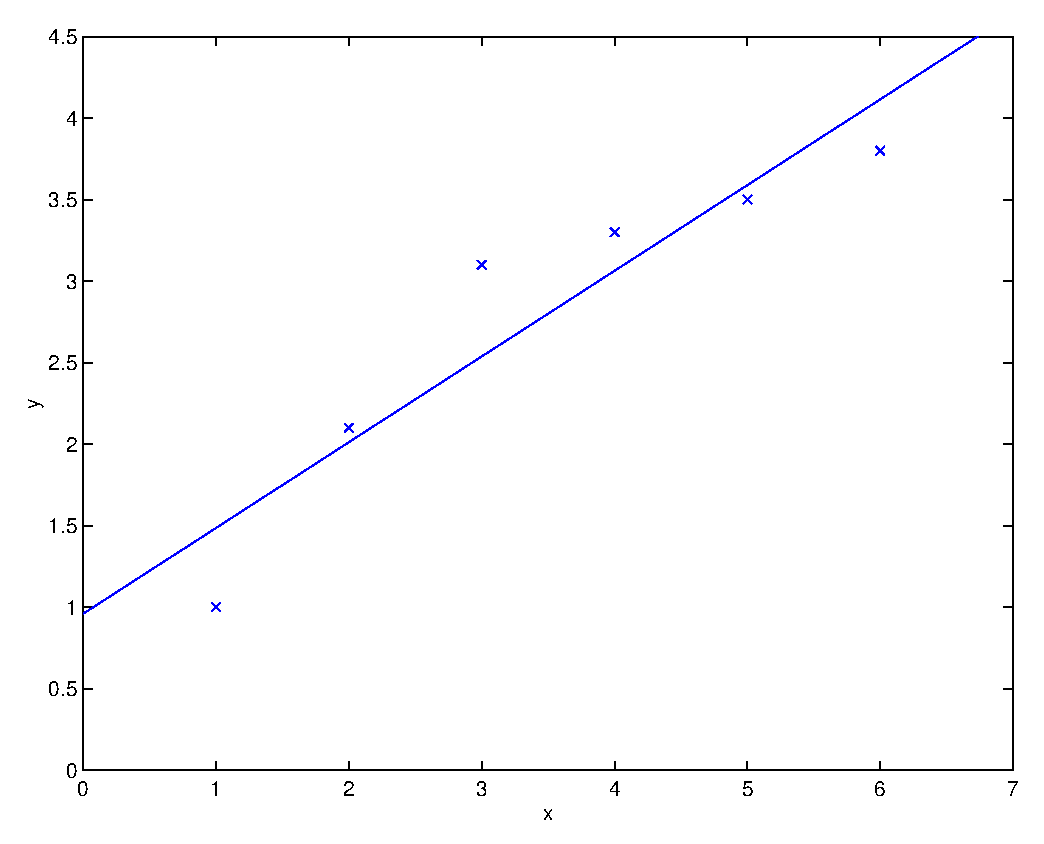
\includegraphics[width=.3\textwidth]{regressionPoly1.eps}\hfill
  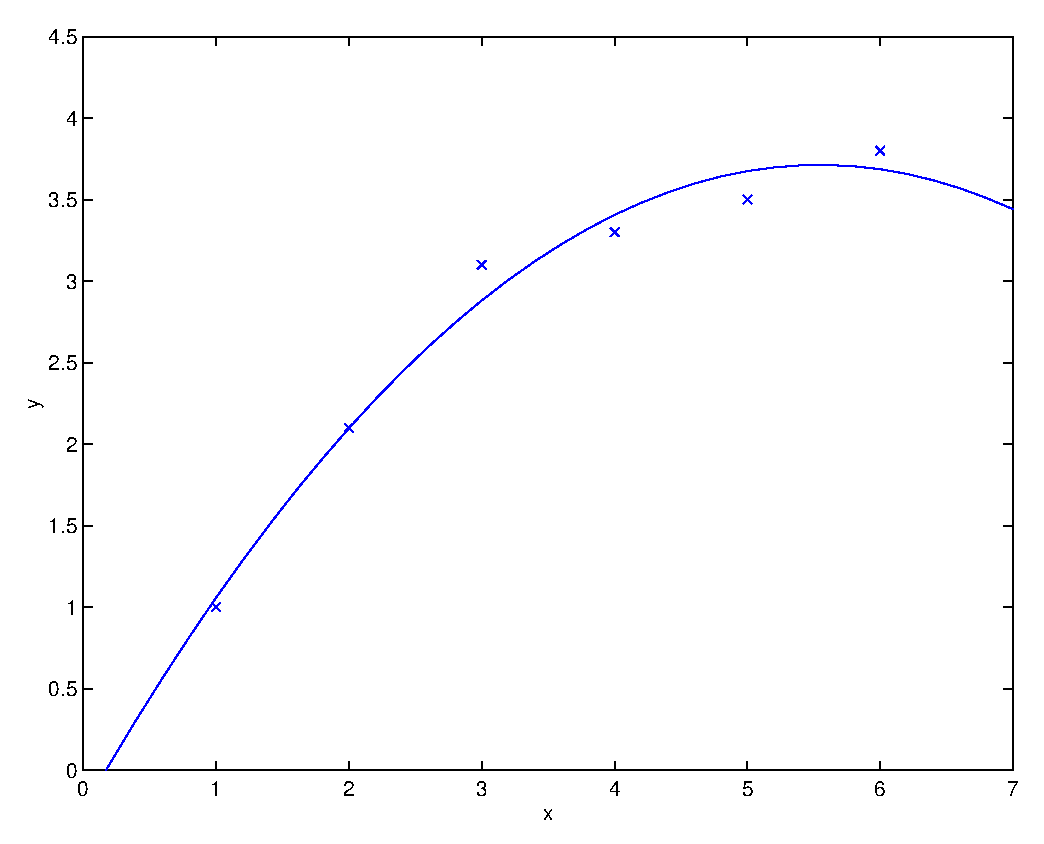
\includegraphics[width=.3\textwidth]{regressionPoly2.eps}\hfill
  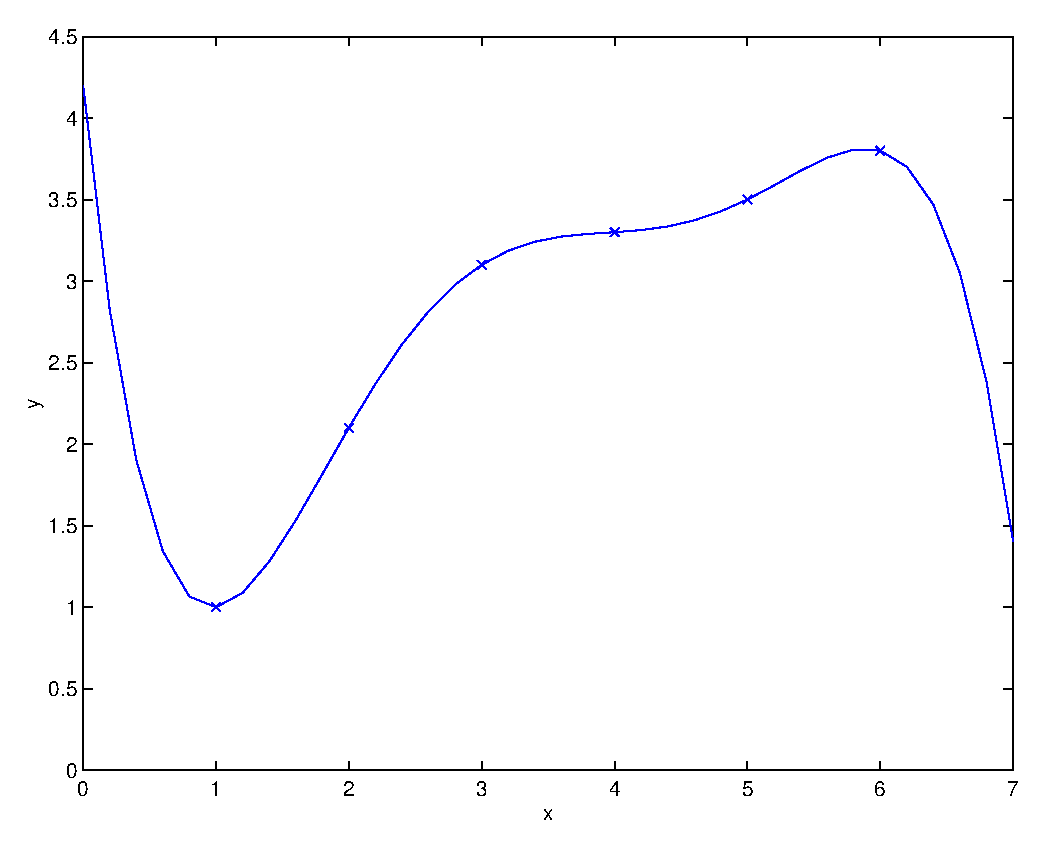
\includegraphics[width=.3\textwidth]{regressionPoly5.eps}
\end{center}

Fitting a 5th order polynomial to the data (rightmost figure) did not result in a good
model.  Specifically, even though the 5th order polynomial did a very good job
predicting $y$ (say, prices of houses) from $x$ (say, living area) for the examples
in the training set, we do not expect the model shown to be a good one for predicting
the prices of houses not in the training set.  In other words, what has been
learned from the training set does not \emph{generalize} well to other houses.
The {\bf generalization error} (which will be made formal shortly)
of a hypothesis is its expected error on examples not necessarily in the
training set.

Both the models in the leftmost and the rightmost figures above have large
generalization error.  However, the problems that the two models suffer from
are very different.  If the relationship between $y$ and $x$ is not linear,
then even if we were fitting a linear model to a very large amount of training
data, the linear model would still fail to accurately capture the structure
in the data.  Informally, we define the {\bf bias} of a model to be the
expected generalization error even if we were to fit it to a very (say,
infinitely) large training set.  Thus, for the problem above, the linear
model suffers from large bias, and may underfit (i.e., fail to capture
structure exhibited by) the data.

Apart from bias, there's a second component to the generalization error,
consisting of the {\bf variance} of a model fitting procedure.  Specifically,
when fitting a 5th order polynomial as in the rightmost figure, there is a
large risk that we're fitting patterns in the data that happened to be
present in our small, finite training set, but that do not reflect the
wider pattern of the relationship between $x$ and $y$.   This could be,
say, because in the
training set we just happened by chance to get a slightly more-expensive-than-average
house here, and a slightly less-expensive-than-average house there, and so on.
By fitting these ``spurious'' patterns in the training set, we might again
obtain a model with large generalization error.  In this case, we say the
model has large variance.\footnote{In these notes, we will not try to
formalize the definitions of bias and variance beyond this discussion.
While bias and variance
are straightforward to define formally for, e.g., linear regression,
there have been several proposals for the definitions of bias and
variance for classification, and there is as yet no agreement on what is
the ``right'' and/or the most useful formalism.}

Often, there is a tradeoff between bias and variance.
If our model is too ``simple'' and has very few parameters, then it may have large
bias (but small variance); if it is too ``complex'' and has very many parameters,
then it may suffer from large variance (but have smaller bias).  In the example above,
fitting a quadratic function does better than either of the extremes of a first
or a fifth order polynomial.

\section{Preliminaries}

In this set of notes, we begin our foray into learning theory.  Apart from being
interesting and enlightening in its own right, this discussion will also help us
hone our intuitions and derive rules of thumb about how to best apply learning algorithms
in different settings.  We will also seek to answer a few questions:  First, can we
make formal the bias/variance tradeoff that was just discussed?
This will also eventually lead us to talk about model selection methods, which can,
for instance, automatically decide what order polynomial to fit to a training set.
Second, in machine learning it's really generalization error
that we care about, but most learning algorithms fit their models
to the training set. Why should doing well on the training set tell us anything
about generalization error?  Specifically, can we relate error on the training
set to generalization error?  Third and finally, are there conditions under
which we can actually prove that learning algorithms will work well?

We start with two simple but very useful lemmas.

\medskip
\noindent
{\bf Lemma.} (The union bound).  Let $A_1, A_2, \ldots, A_k$ be $k$ different
events (that may not be independent).  Then
\[
P(A_1 \cup \cdots \cup A_k) \leq P(A_1) + \ldots + P(A_k).
\]

In probability theory, the union bound is usually stated as an axiom
(and thus we won't try to prove it), but it also makes intuitive sense: The probability of
any one of $k$ events happening is at most the sum of the probabilities of the $k$
different events.

\medskip
\noindent
{\bf Lemma.} (Hoeffding inequality)  Let $Z_1, \ldots, Z_{\nexp}$ be $\nexp$
independent and identically distributed (iid) random variables drawn from
a Bernoulli($\phi$) distribution.  I.e., $P(Z_i = 1) = \phi$, and $P(Z_i=0) = 1-\phi$.
Let $\phihat = (1/\nexp) \sum_{i=1}^\nexp Z_i$ be the mean of these random variables,
and let any $\gamma > 0$ be fixed.  Then
\[
P(|\phi - \phihat| > \gamma) \leq 2 \exp(-2\gamma^2 \nexp)
\]

This lemma (which in learning theory is also called the {\bf Chernoff bound})
says that if we take $\phihat$---the average of $\nexp$
Bernoulli($\phi$) random variables---to be our estimate of $\phi$, then the
probability of our being far from the true value is small, so long as $\nexp$ is
large.  Another way of saying this is that if you have a biased coin whose
chance of landing on heads is $\phi$, then if you toss it $\nexp$ times and
calculate the fraction of times that it came up heads, that will be a
good estimate of $\phi$ with high probability (if $\nexp$ is large).

Using just these two lemmas, we will be able to prove some
of the deepest and most important results in learning theory.

To simplify our exposition, let's restrict our attention to binary
classification in which the labels are $y \in \{0,1\}$.  Everything we'll
say here generalizes to other problems, including regression and multi-class
classification.

We assume we are given a training set $S = \{(\xsi, \ysi); i=1,\ldots,\nexp\}$ of size $\nexp$,
where the training examples $(\xsi, \ysi)$ are drawn iid from
some probability distribution ${\cal D}$.  For a hypothesis $h$, we define the
{\bf training error} (also called the {\bf empirical risk} or {\bf empirical error}
in learning theory) to be
\[
\ehat(h) = \frac{1}{\nexp}\sum_{i=1}^\nexp 1\{h(\xsi) \neq \ysi\}.
\]
This is just the fraction of training examples that $h$ misclassifies.
When we want to make explicit the dependence of $\ehat(h)$ on the training set $S$,
we may also write this a $\hat\varepsilon_S(h)$.
We also define the generalization error to be
\[
\varepsilon(h) = P_{(x,y)\sim {\cal D}}(h(x) \neq y).
\]
I.e. this is the probability that, if we now draw a new example $(x,y)$ from the distribution
${\cal D}$, $h$ will misclassify it.

Note that we have assumed that the training data was drawn from the \emph{same}
distribution $\calD$ with which we're going to evaluate our hypotheses
(in the definition of generalization error).  This is
sometimes also referred to as one of the {\bf PAC} assumptions.\footnote{PAC stands
for ``probably approximately correct,'' which is a framework and set of assumptions
under which numerous results on learning theory were proved.  Of these, the
assumption of training and testing on the same distribution, and the assumption
of the independently drawn training examples, were the most important.}

Consider the setting of linear classification, and let $h_\theta(x) = 1\{\theta^Tx \geq 0\}$.
%Note that, even if we were using an algorithm like logistic regression that tries to
%model $p(y|x)$, if at the end of the day we're asked to make a 0/1 prediction, then we
%would threshold $p(y|x)$ at 0.5 anyway, and this is the form that would be taken
%by map from $x$'s to our predictions.
What's a reasonable way of fitting the parameters $\theta$?
One approach is to try to minimize the training error, and pick
\[
\hat\theta = \arg \min_\theta \ehat(h_\theta).
\]
We call this process {\bf empirical risk minimization} (ERM), and the resulting
hypothesis output by the learning algorithm is $\hhat = h_{\hat\theta}$.
We think of ERM as the most ``basic'' learning algorithm, and it will be this
algorithm that we focus on in these notes.  (Algorithms such as logistic
regression can also be viewed as approximations to empirical risk minimization.)

In our study of learning theory, it will be useful to abstract away
from the specific parameterization of hypotheses and from issues such
as whether we're using a
linear classifier.  We define the {\bf hypothesis class} $\calH$ used by a learning
algorithm to be the set of all classifiers considered by it. For linear
classification, $\calH = \{ h_\theta : h_\theta(x) = 1\{\theta^Tx\geq0\}, \theta \in \Re^{\di+1}\}$
is thus the set of all classifiers over $\calX$
(the domain of the inputs)
where the decision boundary is linear.
More broadly, if we were studying, say, neural networks, then we could let $\calH$ be
the set of all classifiers representable by some neural network architecture.

Empirical risk minimization can now be thought of as a minimization over the class
of functions $\calH$, in which the learning algorithm picks the hypothesis:
\[
\hhat = \arg \min_{h \in \calH} \ehat(h)
\]

\section{The case of finite $\calH$}

Let's start by considering a learning problem in which we have a finite hypothesis
class $\calH = \{h_1, \ldots, h_k\}$ consisting of $k$ hypotheses.  Thus, $\calH$
is just a set of $k$ functions mapping from $\calX$
to
$\{0,1\}$, and empirical risk minimization selects $\hhat$ to be whichever of these $k$ functions
has the smallest training error.

We would like to give guarantees on the generalization error of $\hhat$.
Our strategy for doing so will be in two parts: First, we will show that $\ehat(h)$ is
a reliable estimate of $\varepsilon(h)$ for all $h$.  Second, we will show that
this implies an upper-bound on the generalization error of $\hhat$.

Take any one, fixed, $h_i \in \calH$.  Consider a Bernoulli random variable $Z$ whose
distribution is defined as follows.  We're going to sample $(x, y) \sim {\cal D}$.
Then, we set $Z = 1\{h_i(x) \neq y\}$.  I.e., we're going to draw one example,
and let $Z$ indicate whether $h_i$ misclassifies it.  Similarly, we also
define $Z_j = 1\{h_i(x^{(j)}) \neq y^{(j)}\}$.  Since our training set was drawn iid from $\calD$,
$Z$ and the $Z_j$'s have the same distribution.

We see that the misclassification probability on a randomly drawn
example---that is, $\varepsilon(h)$---is exactly the expected value
of $Z$ (and $Z_j$).  Moreover, the training error can be written
\[
\ehat(h_i) = \frac{1}{\nexp} \sum_{j=1}^\nexp Z_j.
\]
Thus, $\ehat(h_i)$ is exactly the mean of the $\nexp$ random variables $Z_j$ that are
drawn iid from a Bernoulli distribution with mean $\varepsilon(h_i)$.
Hence, we can apply the Hoeffding inequality, and obtain
\[
P(|\varepsilon(h_i) - \ehat(h_i)| > \gamma) \leq 2\exp(-2\gamma^2\nexp).
\]

This shows that, for our particular $h_i$, training error will be close
to generalization error with high probability, assuming $\nexp$ is large.
But we don't just want to guarantee that $\varepsilon(h_i)$ will be close to $\ehat(h_i)$ (with
high probability) for just only one particular $h_i$.  We want to prove that this will be true
simultaneously for \emph{all} $h \in \calH$.  To do so, let $A_i$ denote the event that
$|\varepsilon(h_i) - \ehat(h_i)| > \gamma$.  We've already shown that, for any particular $A_i$,
it holds true that $P(A_i) \leq 2\exp(-2\gamma^2\nexp)$.  Thus, using the union bound, we have
that
\begin{eqnarray*}
P(\exists\, h \in \calH. |\varepsilon(h_i) - \ehat(h_i)| > \gamma)
&=& P(A_1 \cup \cdots \cup A_k) \\
&\leq& \sum_{i=1}^k P(A_i) \\
&\leq& \sum_{i=1}^k 2\exp(-2\gamma^2\nexp)\\
&=& 2k\exp(-2\gamma^2\nexp)
\end{eqnarray*}
If we subtract both sides from 1, we find that
\begin{eqnarray*}
P(\neg \exists\, h \in \calH. |\varepsilon(h_i) - \ehat(h_i)| > \gamma)
&=& P(\forall h \in \calH. |\varepsilon(h_i) - \ehat(h_i)| \leq \gamma) \\
&\geq& 1-2k\exp(-2\gamma^2\nexp)
\end{eqnarray*}
(The ``$\neg$'' symbol means ``not.'') So, with probability
at least $1-2k\exp(-2\gamma^2\nexp)$, we have that
$\varepsilon(h)$ will be within $\gamma$ of $\ehat(h)$ for all $h \in \calH$.  This is
called a \emph{uniform convergence} result, because this is a bound that holds
simultaneously for all (as opposed to just one) $h \in \calH$.

In the discussion above, what we did was, for particular values
of $\nexp$ and $\gamma$, give a bound on
the probability that for some $h \in \calH$,  $|\varepsilon(h) - \ehat(h)| > \gamma$.
There are three quantities of interest here: $\nexp$, $\gamma$, and the probability of
error; we can bound either one in terms of the other two.

For instance, we can ask the following question: Given $\gamma$ and some $\delta > 0$,
how large must $\nexp$ be before we can guarantee that with probability at least $1-\delta$, training
error will be within $\gamma$ of generalization error?
By setting $\delta = 2k\exp(-2\gamma^2\nexp)$ and solving for $\nexp$,
[you should convince yourself this is the right thing to do!],
we find that if
\[
\nexp \geq \frac{1}{2\gamma^2} \log \frac{2k}{\delta},
\]
then with probability at least $1-\delta$,  we have that $|\varepsilon(h) - \ehat(h)| \leq \gamma$
for all $h \in \calH$.  (Equivalently, this shows that the probability that
$|\varepsilon(h) - \ehat(h)| > \gamma$ for some $h \in \calH$ is at most $\delta$.)
This bound tells us how many training examples we need in order make
a guarantee.  The training set size $\nexp$ that a certain method or algorithm
requires in order to achieve a certain level of performance is also called
the algorithm's {\bf sample complexity}.

The key property of the bound above is that the number of training examples
needed to make this guarantee is only \emph{logarithmic} in $k$,
the number of hypotheses in $\calH$.  This will be important later.

Similarly, we can also hold $\nexp$ and $\delta$ fixed and solve for $\gamma$
in the previous equation,
and show [again, convince yourself that this is right!] that with probability $1-\delta$, we
have that for all $h \in \calH$,
\[
|\ehat(h) - \varepsilon(h)| \leq \sqrt{\frac{1}{2\nexp}\log\frac{2k}{\delta}}.
\]

Now, let's assume that uniform convergence holds, i.e., that
$|\varepsilon(h) - \ehat(h)| \leq \gamma$ for all $h \in \calH$.  What can we prove about
the generalization of our learning algorithm that picked $\hhat = \arg \min_{h \in \calH}\ehat(h)$?

Define $\hstar = \arg \min_{h \in \calH} \varepsilon(h)$ to be the best possible hypothesis in $\calH$.
Note that $\hstar$ is the best that we could possibly do given that we are using $\calH$, so it
makes sense to compare our performance to that of $\hstar$. We have:
\begin{eqnarray*}
\varepsilon(\hhat) &\leq& \ehat(\hhat) + \gamma  \\
&\leq& \ehat(\hstar) + \gamma  \\
&\leq& \varepsilon(\hstar) + 2\gamma
\end{eqnarray*}
The first line used the fact that $|\varepsilon(\hhat) -\ehat(\hhat)| \leq \gamma$ (by our uniform
convergence assumption). The second used the fact that $\hhat$ was chosen to minimize $\ehat(h)$,
and hence $\ehat(\hhat) \leq \ehat(h)$ for all $h$, and in particular
$\ehat(\hhat) \leq \ehat(\hstar)$.  The third line used the uniform convergence assumption again,
to show that $\ehat(\hstar) \leq \varepsilon(\hstar) + \gamma$.  So, what
we've shown is the following: If uniform convergence occurs,
then the generalization error of $\hhat$ is at
most $2\gamma$ worse than the best possible hypothesis in $\calH$!

Let's put all this together into a theorem.

\medskip
\noindent
{\bf Theorem.}  Let $|\calH| = k$, and let any $\nexp, \delta$ be fixed.  Then with probability
at least $1-\delta$, we have that
\[
\varepsilon(\hhat) \leq \left( \min_{h \in \calH} \varepsilon(h) \right) + 2 \sqrt{\frac{1}{2\nexp}\log\frac{2k}{\delta}}.
\]
\medskip

This is proved by letting $\gamma$ equal the $\sqrt{\cdot}$ term, using our previous argument
that uniform convergence occurs with probability at least $1-\delta$, and
then noting that uniform convergence implies $\varepsilon(h)$ is at
most $2\gamma$ higher than $\varepsilon(\hstar) = \min_{h \in \calH} \varepsilon(h)$
(as we showed previously).

This also quantifies what we were saying previously saying about the bias/variance tradeoff in model
selection.  Specifically, suppose we have some hypothesis class $\calH$, and are
considering switching to some much larger hypothesis class $\calH' \supseteq \calH$.
If we switch to $\calH'$, then the first term
$\min_h \varepsilon(h)$ can only decrease (since we'd then be taking a min
over a larger set of functions).  Hence,
by learning using a larger hypothesis class, our ``bias'' can only
decrease.  However, if k increases, then the second $2\sqrt{\cdot}$ term
would also increase.  This increase corresponds to our ``variance'' increasing
when we use a larger hypothesis class.

By holding $\gamma$ and $\delta$ fixed and solving for $\nexp$ like we
did before, we can also obtain the following sample complexity bound:

\medskip
\noindent
{\bf Corollary.} Let $|\calH|=k$, and let any $\delta, \gamma$ be fixed.  Then for
$\varepsilon(\hhat) \leq \min_{h \in \calH} \varepsilon(h) + 2 \gamma$ to hold with probability at least $1-\delta$,
it suffices that
\begin{eqnarray*}
\nexp &\geq& \frac{1}{2\gamma^2}\log\frac{2k}{\delta}\\
  &=& O\left(\frac{1}{\gamma^2}\log\frac{k}{\delta}\right),
\end{eqnarray*}


\section{The case of infinite $\calH$}

We have proved some useful theorems for the case of finite hypothesis
classes. But many hypothesis classes, including any parameterized by real numbers
(as in linear classification) actually contain an infinite number of functions.
Can we prove similar results for this setting?

Let's start by going through something that is \emph{not} the ``right'' argument.
\emph{Better and more general arguments exist}, but this will be useful for
honing our intuitions about the domain.

Suppose we have an $\calH$ that is parameterized by $\di$ real numbers.  Since we are using a computer to
represent real numbers, and IEEE double-precision floating point ({\tt double}'s in C)
uses 64 bits
to represent a floating point number, this means that our learning algorithm, assuming we're using
double-precision floating point,  is parameterized by $64\di$ bits.  Thus, our hypothesis class
really consists of at most $k=2^{64\di}$ different hypotheses.  From the Corollary at the end of the
previous section, we therefore find that, to guarantee
$\varepsilon(\hhat) \leq \varepsilon(\hstar) + 2 \gamma$, with to hold with probability at least $1-\delta$,
it suffices that
$\nexp \geq O\left(\frac{1}{\gamma^2}\log\frac{2^{64\di}}{\delta}\right)
= O\left(\frac{\di}{\gamma^2}\log\frac{1}{\delta}\right)
= O_{\gamma,\delta}(\di)$.  (The $\gamma,\delta$ subscripts indicate that the last big-$O$ is hiding constants that may
depend on $\gamma$ and $\delta$.)  Thus, the number of training examples needed is at most \emph{linear}
in the parameters of the model.

The fact that we relied on 64-bit floating point makes this argument not entirely satisfying,
but the conclusion is nonetheless roughly correct: If what we try to do is minimize training error,
then in order to learn ``well'' using a hypothesis class that has $\di$ parameters, generally we're
going to need on the order of a linear number of training examples in $\di$.

(At this point, it's worth noting that these results were proved for an algorithm
that uses empirical risk minimization.  Thus, while the linear dependence of sample
complexity on $\di$ does generally
hold for most discriminative learning algorithms that try to minimize training
error or some approximation to training error, these conclusions do not
always apply as readily to discriminative learning algorithms.  Giving good theoretical
guarantees on many non-ERM learning algorithms is still an area of
active research.)
% fall into this category, but these conclusions do not always apply to
%generative learning algorithms.)

%learning Note that there're also learning algorithms that are very different from the ones we've seen so far,
%and in particular do not try to minimize training error.  Some of these algorithms, such as support vector
%machines (SVMs), might require far fewer training examples that $O(d)$, but we won't have time to cover them
%in this class.)

The other part of our previous argument that's slightly unsatisfying is that
it relies on the parameterization of $\calH$.
Intuitively, this doesn't seem like it should matter: We had written the class
of linear classifiers as
$h_\theta(x) = 1\{\theta_0 + \theta_1 x_1 + \cdots \theta_{\di} x_{\di} \geq 0\}$,
with $n+1$ parameters $\theta_0, \ldots, \theta_{\di}$.
But it could also be written
$h_{u,v}(x) = 1\{(u^2_0 - v^2_0) + (u^2_1 - v^2_1) x_1 + \cdots (u^2_{\di} - v^2_{\di}) x_{\di} \geq 0\}$ with $2\di+2$ parameters $u_i, v_i$.
Yet, both of these are just defining the same $\calH$: The set of linear classifiers in $\di$ dimensions.

To derive a more satisfying argument, let's define a few more things.

Given a set $S = \{\xsi, \ldots, \xsvcd\}$ (no relation to the training set)
of points $\xsi \in \calX$, we say that $\calH$ {\bf shatters} $S$ if $\calH$ can realize any
labeling on $S$. I.e., if for any set of labels $\{y^{(1)}, \ldots, y^{(\vcd)}\}$,
there exists
some $h \in \calH$ so that $h(\xsi) = \ysi$ for all $i=1,\ldots \vcd$.

Given a hypothesis class $\calH$, we then define its {\bf Vapnik-Chervonenkis dimension},
  written ${\rm VC}(\calH)$, to be the
size of the largest set that is shattered by $\calH$.  (If $\calH$ can shatter arbitrarily large sets, then
${\rm VC}(\calH) = \infty$.)

For instance, consider the following set of three points:

\begin{center}
% eps library outdated
% \epsfxsize=2in
% \epsffile{shatter3.eps}
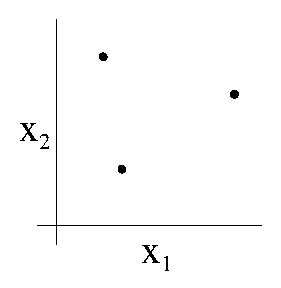
\includegraphics[scale=0.5]{shatter3.eps}
\end{center}

Can the set $\calH$ of linear classifiers in two
dimensions ($h(x) = 1\{\theta_0 + \theta_1 x_1 + \theta_2 x_2\geq 0 \}$) can shatter
the set above?  The answer is yes.  Specifically, we see that, for any of the eight possible
labelings of these points, we can find a linear classifier that obtains ``zero training error''
on them:
\begin{center}
% eps library outdated
% \epsfxsize=5in
% \epsffile{shatter3-8.eps}
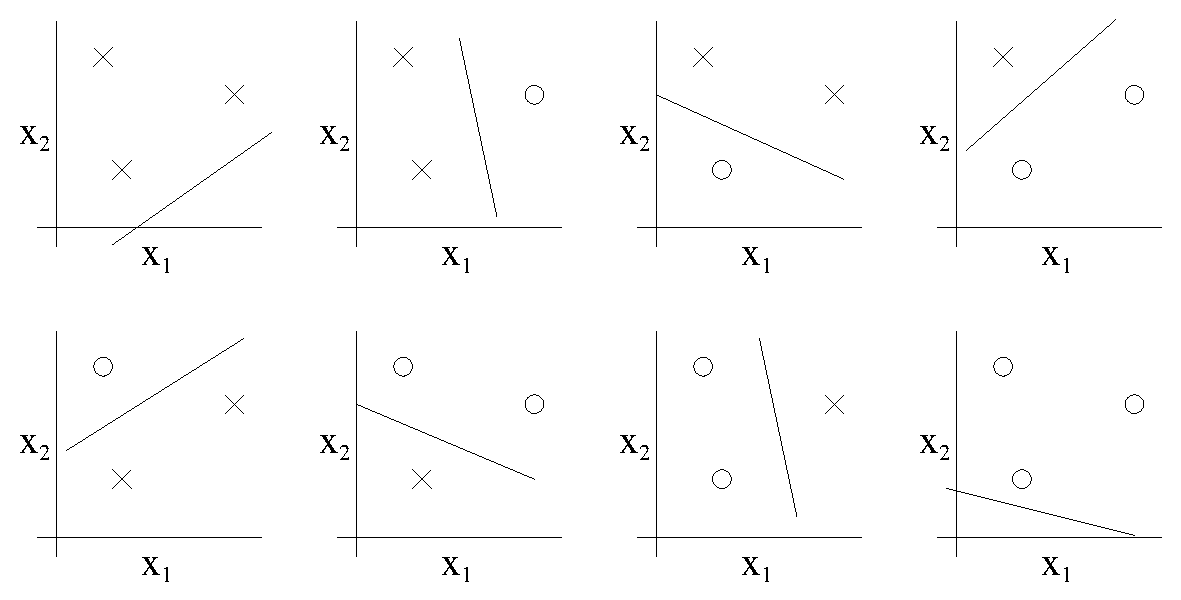
\includegraphics[scale=0.5]{shatter3-8.eps}
\end{center}
Moreover, it is possible to show that there is no set of 4 points that this
hypothesis class can shatter.  Thus, the largest set that $\calH$ can shatter
is of size 3, and hence ${\rm VC}(\calH)=3$.

Note that the VC dimension of $\calH$ here is 3 even though there may be sets of
size 3 that it cannot shatter.  For instance, if we had a set of three points
lying in a straight line (left figure), then there is no way to find a
linear separator for the labeling of the three points shown below (right figure):
\begin{center}
% eps library outdated
% \epsfxsize=5in
% \epsffile{collinear-notshatter.eps}
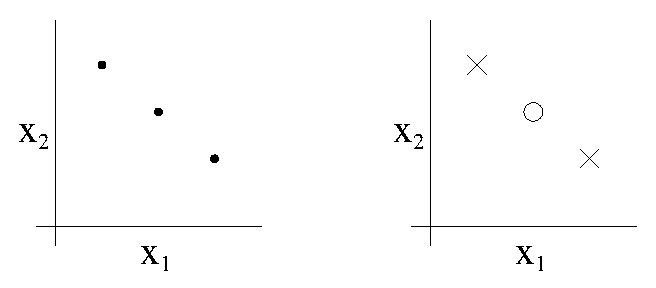
\includegraphics[scale=0.5]{collinear-notshatter.eps}
\end{center}

In order words, under the definition of the VC dimension, in order to prove that
$\VC(\calH)$ is at least $\vcd$, we need to show only
that there's at least \emph{one} set of size $\vcd$ that $\calH$ can shatter.

The following theorem, due to Vapnik, can then be shown.  (This is, many would argue,
the most important theorem in all of learning theory.)

\noindent
{\bf Theorem.}
Let $\calH$ be given, and let $\vcd = {\rm VC}(\calH)$.  Then with probability at least $1-\delta$, we
have that for all $h \in \calH$,
\[
|\varepsilon(h) - \ehat(h)| \leq O\left(\sqrt{\frac{\vcd}{\nexp}\log\frac{\nexp}{\vcd} + \frac{1}{\nexp}\log\frac{1}{\delta}}\right).
\]
Thus, with probability at least $1-\delta$, we also have that:
\[
\varepsilon(\hhat) \leq \varepsilon(\hstar) + O\left(\sqrt{\frac{\vcd}{\nexp}\log\frac{\nexp}{\vcd} + \frac{1}{\nexp}\log\frac{1}{\delta}}\right).
\]

In other words, if a hypothesis class has finite VC dimension,
then uniform convergence occurs as $\nexp$ becomes large.
As before,
this allows us to give a bound on $\varepsilon(h)$ in terms
of $\varepsilon(\hstar)$.  We also
have the following corollary:

\medskip
\noindent
{\bf Corollary.}  For $|\varepsilon(h) - \ehat(h)| \leq \gamma$ to hold for all $h \in \calH$
(and hence $\varepsilon(\hhat) \leq \varepsilon(\hstar) + 2\gamma$) with probability at least $1-\delta$,
it suffices that $\nexp = O_{\gamma,\delta}(\vcd)$.
\medskip

In other words, the number of training examples needed to learn ``well'' using $\calH$ is linear
in the VC dimension of $\calH$.  It turns out that, for ``most'' hypothesis classes, the VC dimension
(assuming a ``reasonable'' parameterization) is also roughly linear in the number of parameters.
Putting these together, we conclude that for a given hypothesis class $\calH$ (and for an algorithm that
tries to minimize training error), the number of training
examples needed to achieve generalization error close to that of the optimal classifier is usually roughly linear in the number of parameters of $\calH$.

\end{document}


